\documentclass{beamer}
\usetheme{Boadilla}
\usepackage{graphicx}
\usepackage[normalem]{ulem}

% -- ChatGPTeries pour slide dorée --%
\usepackage{tikz}
\usepackage{xcolor}

\definecolor{gold}{RGB}{201, 164, 76}
\definecolor{darkgold}{RGB}{142, 111, 35}
\definecolor{luxuryblack}{RGB}{18, 18, 18}
\definecolor{softwhite}{RGB}{242, 240, 234}
% ---- %

\usepackage{tikz}
\usepackage{xcolor}
\usetikzlibrary{positioning, calc}

% -- Icones pour la slide "langage de haut niveau" -- %
% Baguette magique : image demandee par l'utilisateur (istockphoto, a
% verifier niveau licence avant toute diffusion publique des slides).
\newcommand{\wandicon}{\reflectbox{
\includegraphics[width=2.5 cm]{Images/baguette_magique.jpg}}}
\newcommand{\screenicon}{%
	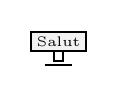
\begin{tikzpicture}[baseline=-0.3ex, scale=0.35]
		\draw[thick, fill=black!5] (-1,0) rectangle (1,0.7);
		\node[font=\tiny] at (0,0.35) {Salut};
		\draw[thick] (-0.15,-0.35) rectangle (0.15,0);
		\draw[thick] (-0.5,-0.5) -- (0.5,-0.5);
	\end{tikzpicture}%
}
% ---- %

% -- Coloration syntaxique du code Python (compatible pdflatex) -- %
\usepackage{listings}
\usepackage{lstlinebgrd}
\definecolor{codekw}{RGB}{0, 0, 180}
\definecolor{codestr}{RGB}{20, 120, 40}
\definecolor{codecom}{RGB}{120, 120, 120}
\lstdefinestyle{python}{
	language=Python,
	basicstyle=\ttfamily\footnotesize,
	keywordstyle=\color{codekw}\bfseries,
	stringstyle=\color{codestr},
	commentstyle=\color{codecom}\itshape,
	showstringspaces=false,
	keepspaces=true,
	columns=fullflexible,
	aboveskip=0pt,
	belowskip=0pt,
	literate={é}{{\'e}}1 {è}{{\`e}}1 {ê}{{\^e}}1 {à}{{\`a}}1 {ç}{{\c c}}1
	{É}{{\'E}}1 {'}{{\textquotesingle}}1,
}
\lstdefinestyle{pythonsmall}{style=python,basicstyle=\ttfamily\scriptsize}

% Convention du cours pour une reponse de Python (a la suite d'un print, etc.) :
% prefixe ">" + encadre sur fond clair.
\lstdefinestyle{pythonoutput}{
	style=python,
	basicstyle=\ttfamily\footnotesize\color{black!70},
	backgroundcolor=\color{black!6},
	frame=single,
	rulecolor=\color{black!35},
	framerule=0.4pt,
	framexleftmargin=5pt,
	framexrightmargin=5pt,
	framextopmargin=3pt,
	framexbottommargin=3pt,
	xleftmargin=5pt,
	xrightmargin=5pt,
	aboveskip=3pt,
	belowskip=3pt,
}

% Un morceau de code annote : #1 plage de lignes, #2 1 si c'est la partie
% commentee (fond bleu, couleurs normales) sinon 0 (grise), #3 aboveskip.
\newcommand{\annoline}[3]{%
	\ifnum#2=1
	\lstinputlisting[style=pythonsmall, backgroundcolor=\color{blue!15}, #3, linerange={#1}]{code/premier_prog_2.py}%
	\else
	\lstinputlisting[style=pythonsmall, basicstyle=\ttfamily\scriptsize\color{black!45}, keywordstyle=\color{black!45}, stringstyle=\color{black!45}, #3, linerange={#1}]{code/premier_prog_2.py}%
	\fi
}

% Version generique de \annoline : #1 fichier, #2 plage de lignes,
% #3 1 si c'est la ligne commentee (fond bleu) sinon 0 (grisee).
\newcommand{\valline}[3]{%
	\ifnum#3=1
	\lstinputlisting[style=pythonsmall, backgroundcolor=\color{blue!15}, linerange={#2}]{#1}%
	\else
	\lstinputlisting[style=pythonsmall, basicstyle=\ttfamily\scriptsize\color{black!45}, keywordstyle=\color{black!45}, stringstyle=\color{black!45}, linerange={#2}]{#1}%
	\fi
}

% Slide "focus sur une construction" : etape 1 = programme entier, la partie
% commentee sur fond bleu (texte noir), le reste gris ; etape 2 = le reste a
% disparu, la partie commentee reste sur fond bleu (texte noir).
\newcommand{\focusframe}[5]{%
	\begin{frame}[t]{#1}
		\only<1>{\lstinputlisting[
			style=pythonsmall,
			basicstyle=\ttfamily\scriptsize\color{black!45},
			keywordstyle=\color{black!45}, stringstyle=\color{black!45},
			emph={#2}, emphstyle={\color{black}\bfseries},
			linebackgroundcolor={\color{white}#3},
			]{code/premier_prog_2.py}}%
		\only<2>{\lstinputlisting[
			style=pythonsmall,
			emph={#2}, emphstyle={\color{black}\bfseries},
			linebackgroundcolor={\color{white}#3},
			]{code/#4}}%
		\vfill
		\centering\small #5
	\end{frame}%
}

\title{Algorithmique et Programmation 1}
\author{A. Boussidan, L. Exibard, P. Yvonnet}
\date{14 Septembre 2026}

\begin{document}

\begin{frame}
    \maketitle
\end{frame}

%WOOCLAP 
%Point d'organisation 

\begin{frame}{Organisation globale}

\begin{block}{Planning d'AP1}
Chaque semaine :
    \begin{itemize}
        \item 1 séance de CM 
        \item 1 séance de TD 
        \item 2 séances de TP
            \begin{itemize}
                \item 1 TP "découverte"/entraînement
                \item 1 TP "exo+" : mini-projet, créativité, autonomie,...
            \end{itemize}
    \end{itemize}
    \end{block}
    \pause 
    \begin{center}
        Beaucoup d'heures devant les machines : profitez-en !
    \end{center}
    \end{frame}
   
\begin{frame}{Vos enseignants}
	\only<1>{
		\begin{center}
			Léo Exibard
		\end{center}
	
\includegraphics[width=0.9\textwidth, keepaspectratio=True]{Images/leo_exibard.jpeg}
	\begin{itemize}
		\item Bureau 4B124
		\item leo.exibard@univ-eiffel.fr
		\pause\item Responsable d'AP1 depuis plusieurs années
	\end{itemize}
}
	\only<2>{
	\begin{center}
		Philippe Yvonnet
	\end{center}
	% TODO : photo de Philippe Yvonnet manquante (placeholder {TODO} retire pour compiler)
	\begin{itemize}
		\item Bureau 4B096
		\item philippe.yvonnet@univ-eiffel.fr
		\pause\item Responsable de l'option Projet 1 et de Remédiation
	\end{itemize}
}
	\only<3>{
	\begin{center}
		Aaron Boussidan
	\end{center}
	% TODO : ceci pointait vers leo_exibard.jpeg (copie-colle) - photo d'Aaron a ajouter
	\begin{itemize}
		\item Bureau 4B162
		\item aaron.boussidan@univ-eiffel.fr
		\item Chauve
	\end{itemize}
}	
	
	
\end{frame}
\begin{frame}{Evaluation}

    \begin{block}{Evaluation}
        \begin{itemize}
            \item CC1 la semaine du 02 novembre \only<2->{- \textbf{Coefficient 7 }}
            \item CC2 la semaine du 04 janvier \only<2->{- \textbf{Coefficient 9 }}
            \item TP noté 1 la semaine du 02/10 \only<3->{- \textbf{Coefficient 1.5 }}
            \item TP noté 2 la semaine du 14/12 \only<3->{- \textbf{Coefficient 1.5 }}
            \item Une note de TP \only<4->{- \textbf{Coefficient 1 }}
        \end{itemize}
    \end{block}

    
\end{frame}

\begin{frame}{Bienvenue !}
    \begin{block}{Objectifs de ce cours}
    \begin{itemize}
        \item Découvrir l'informatique et la programmation 
        \item Se (re-)familiariser avec un langage de programmation : Python 
        \item Commencer à penser en \textbf{algorithmes} et pas juste en \textbf{programmes}
    \end{itemize}
    \end{block}
    \pause 
    \vfill
    \begin{block}{A la fin de cours, vous saurez ...}
        \begin{itemize}
            \item Comprendre et écrire des programmes Python simple 
            \item Ecrire un petit jeu vidéo jouable sur une grille (Projet 1 !)
            \item Aborder d'autres langages de programmation
        \end{itemize}
    \end{block}
\end{frame}

\begin{frame}{Liens utiles}
    \large
    \begin{itemize}
        \item Discord de la L1 : \url{https://discord.gg/FSYd7QtxfC}
        \item \href{https://elearning.univ-eiffel.fr/course/view.php?id=16399}{Page Elearning du cours} (avec notes de cours !)
        \item Thonny : \url{https://thonny.org/}
        \item Python Tutor : \url{https://pythontutor.com/}
    \end{itemize}
\end{frame}
    

\begin{frame}{Algorithmique ? Programmation ? }

    \begin{block}{Algorithmique}
        \textbf{Concevoir une solution.}

        
        Quelle est \textbf{l'idée} pour résoudre ce problème ? Quelle \textbf{méthode} utiliser ?  
    \end{block}
    \pause 
    \begin{center}
        Algorithme = recette de cuisine
    \end{center}

    \begin{block}{Programmation}
    \textbf{Exécuter une solution.}

    On "explique" à une machine comment mettre en place la solution.
    Etape par étape, dans un certain \textbf{langage de programmation}.
    \end{block}

    \pause
    \begin{center}
        Programme = cuisiner la recette 
    \end{center}
\end{frame}


% ------------------------------------------------------------------
% Slide "Les règles d'or"
% ------------------------------------------------------------------

\begin{frame}[plain]

\begin{tikzpicture}[remember picture, overlay]

  % Fond
  \fill[luxuryblack] (current page.south west)
      rectangle (current page.north east);

  % Double filet doré, rapproché des bords
  \draw[gold, line width=0.8pt]
      ([xshift=0.28cm,yshift=0.28cm]current page.south west)
      rectangle
      ([xshift=-0.28cm,yshift=-0.28cm]current page.north east);

  \draw[darkgold, line width=0.3pt]
      ([xshift=0.43cm,yshift=0.43cm]current page.south west)
      rectangle
      ([xshift=-0.43cm,yshift=-0.43cm]current page.north east);

  % Petit ornement central
  \node[gold, font=\large] at
      ([yshift=-0.95cm]current page.north)
      {$\diamond$};

  % Titre
  \node[
      anchor=north,
      text=gold,
      font=\fontsize{21}{25}\selectfont\bfseries
  ] at ([yshift=-1.25cm]current page.north)
  {LES RÈGLES D'OR d'AP1};

  % Ligne décorative
  \draw[gold, line width=0.5pt]
      ([xshift=-2.3cm,yshift=-2.15cm]current page.north)
      -- ([xshift=2.3cm,yshift=-2.15cm]current page.north);
\pause
  % ================================================================
  % RÈGLE 01
  % ================================================================

  \node[
      anchor=north west,
      text=gold,
      font=\fontsize{12}{14}\selectfont\bfseries
  ] at ([xshift=1.15cm,yshift=-2.85cm]current page.north west)
  {01};

  \node[
      anchor=north west,
      text=softwhite,
      font=\normalsize\bfseries
  ] at ([xshift=2.05cm,yshift=-2.80cm]current page.north west)
  {Etre un chef.};

  \node[
      anchor=north west,
      text=softwhite!70,
      font=\footnotesize
  ] at ([xshift=2.05cm,yshift=-3.30cm]current page.north west)
  {Penser à l'algorithme avant de programmer};

  % ================================================================
  % Pied de page
  % ================================================================

  \node[
      anchor=south,
      text=gold!80,
      font=\tiny\scshape
  ] at ([yshift=0.75cm]current page.south)
  {À retenir};

\end{tikzpicture}

\end{frame}



\begin{frame}{Soyez des chefs ! }
    \begin{center}
        Pour résoudre un problème en informatique, on commence toujours par penser à \textbf{l'algorithme}.
    \end{center}
\pause
\begin{itemize}
    \item Est-ce que ça ressemble à un problème déjà vu ? 
    \item Quelles étapes pour arriver à la solution ? 
    \item A quoi faut-il faire attention en particulier ? 
\end{itemize}

\pause 
\vfill
\begin{center}
    C'est seulement après qu'on passe en cuisine !
\end{center}

\end{frame}



\begin{frame}{
    \makebox[0.8\textwidth][l]{
\only<1>{"Let me cook"}%
\only<2->{"Let me \sout{cook}\,code"}%
    }
}
\begin{center}
     Dans ce cours on 
    \only<1>{cuisine}
    \only<2->{\sout{cuisine}\,code} en \textbf{Python}.

    \only<1>{
    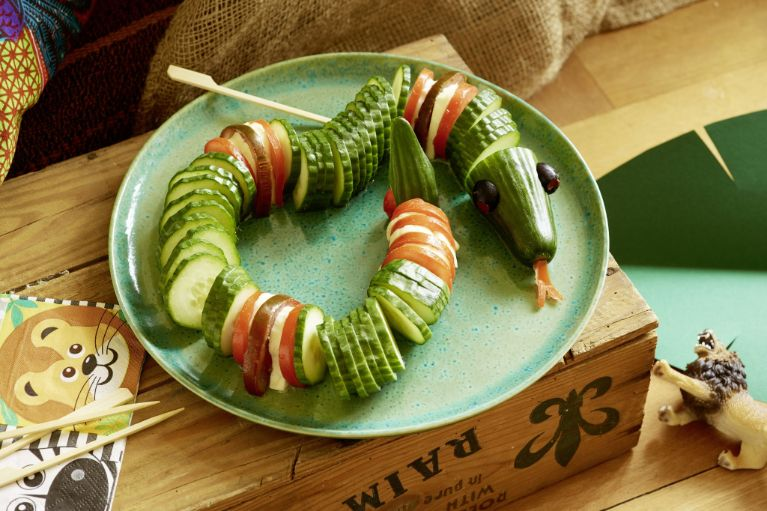
\includegraphics[width = 0.9\textwidth, keepaspectratio=True]{Images/plat-serpent.png}}
    \only<2>{ 
\includegraphics[width = 0.9\textwidth, keepaspectratio=True]{Images/logo_python.png}}
    \uncover<3->{
        Pour démarrer, on va devoir mettre la main à la pâte. \\
        \only<3>{ 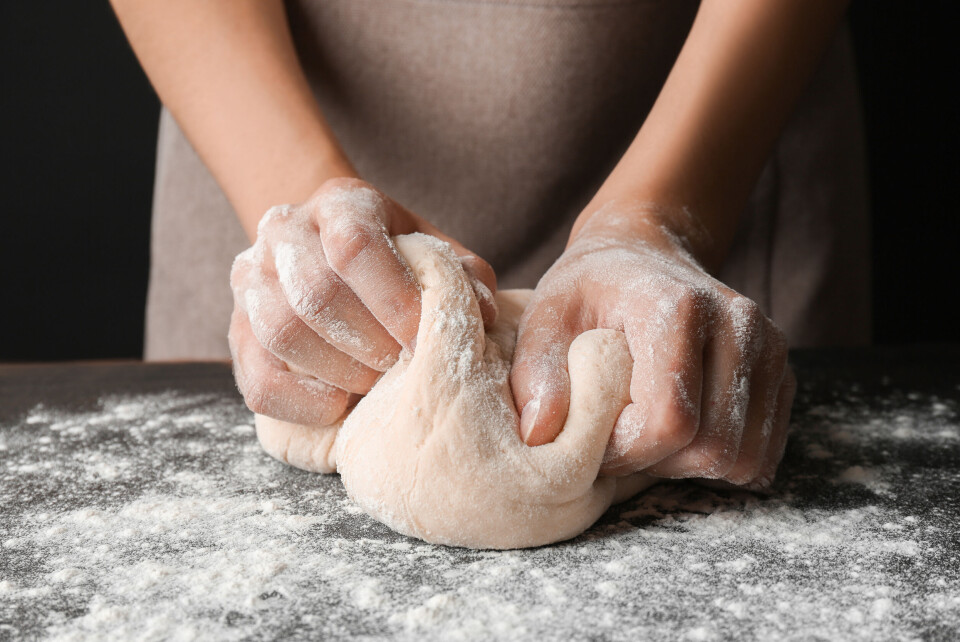
\includegraphics[width = 0.9\textwidth, keepaspectratio=True]{Images/main_a_la_pate.png}}
    }
    \uncover<4->{
         Quand on sera des grands chefs, on aura des commis de cuisine. 
         \only<4>{ 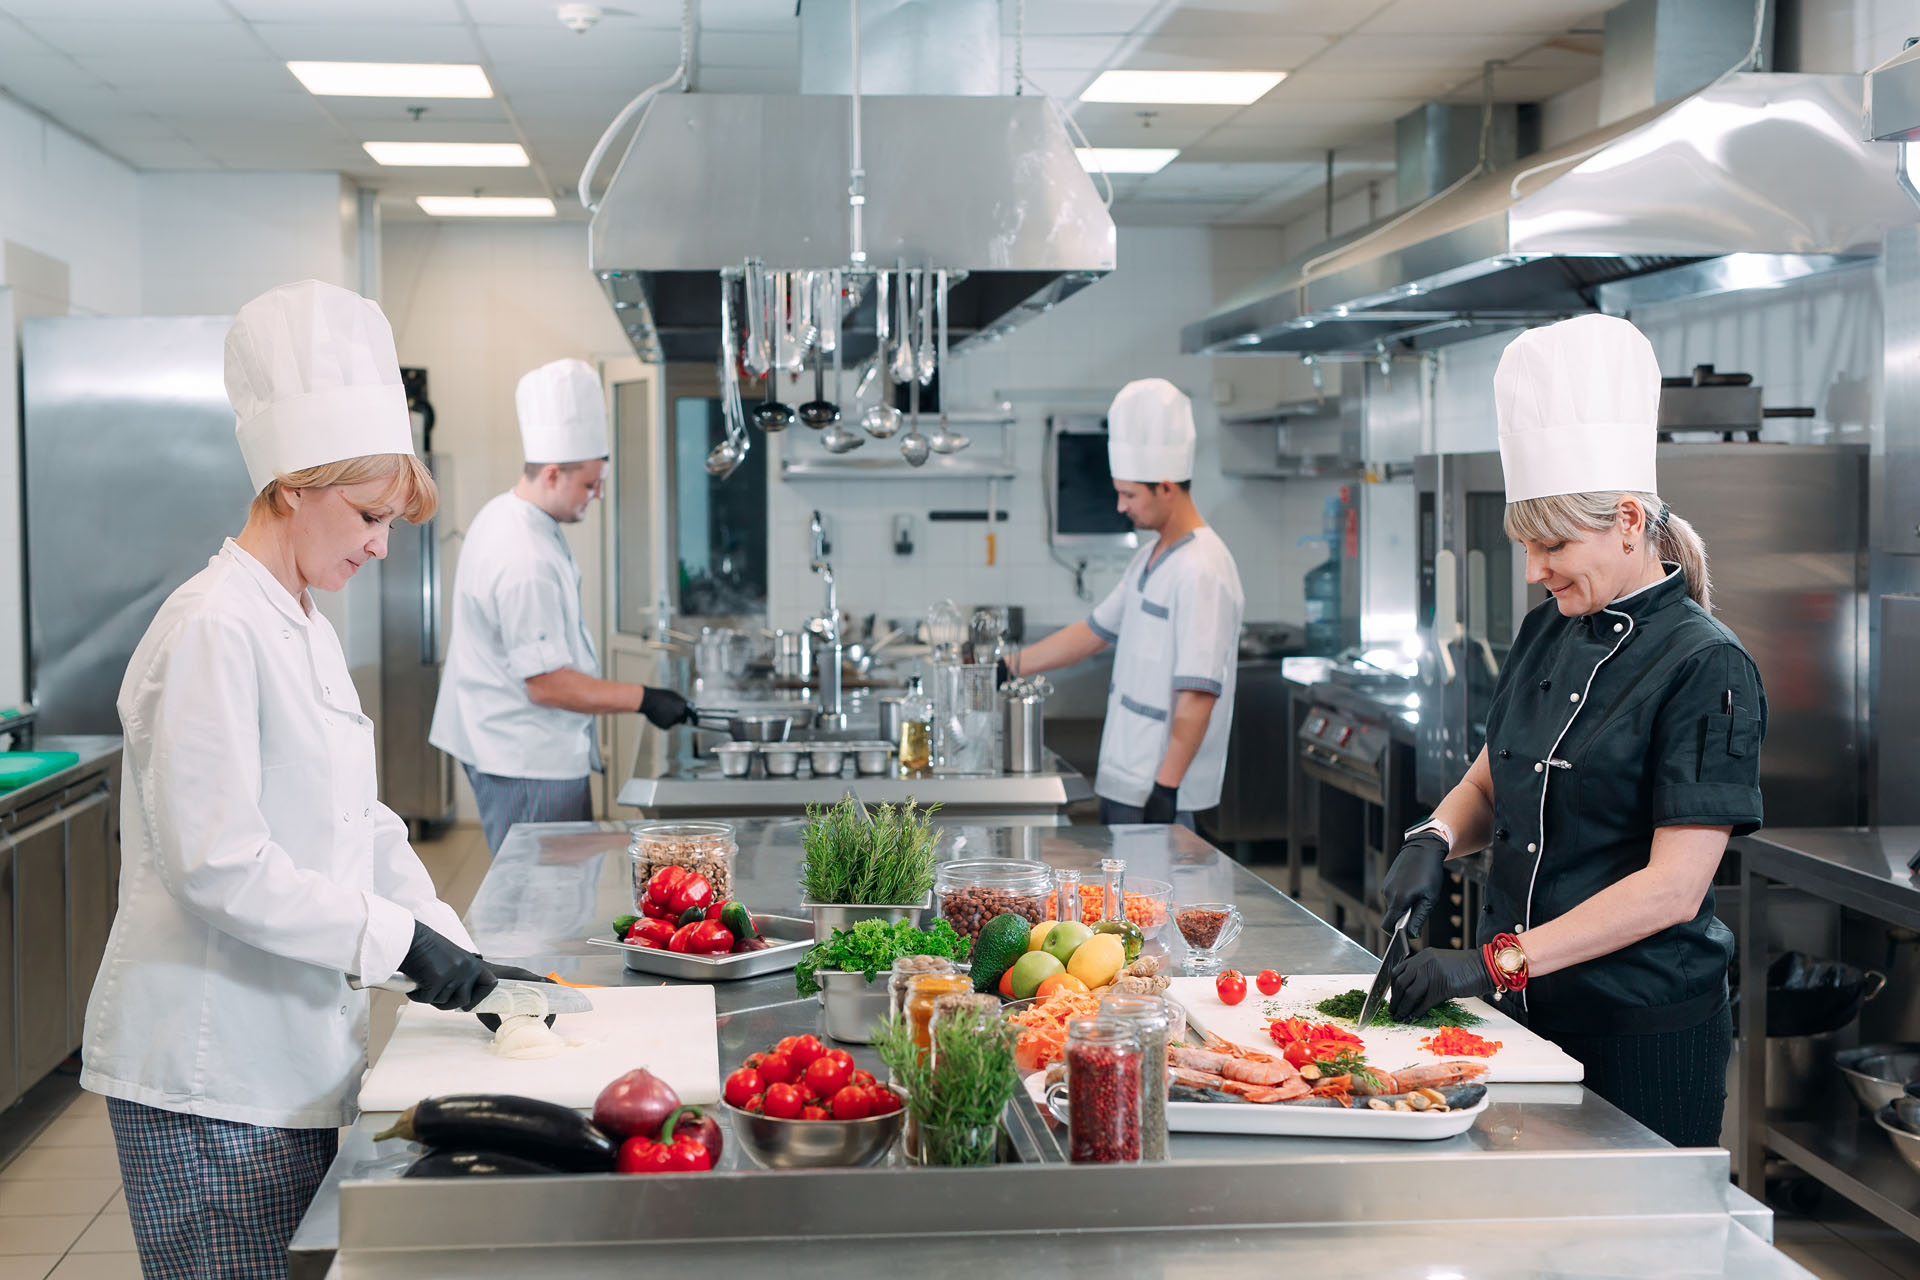
\includegraphics[width = 0.9\textwidth, keepaspectratio=True]{Images/commis_cuisine.png}}
         \only<5>{ 
\includegraphics[width = 0.5\textwidth, keepaspectratio=True]{Images/ChatGPT.png}}
    }
\end{center}
\end{frame}

\begin{frame}[t]{Un langage ``haut niveau''}
	\begin{center}
		\begin{tikzpicture}[every node/.style={font=\small}]
			\node[draw, rounded corners, minimum width=6cm, minimum height=1cm] (py) at (0,5.2)
			{\texttt{print("Salut")}};
			\node[draw, rounded corners, minimum width=6cm, minimum height=1cm] (mach) at (0,0.85)
			{\texttt{01101000 01101001 ...}};
			\node (screen) at (0,-1.4) {\screenicon};
			
			% etapes 1-2 : lien direct (pas de detail)
			\only<1-2>{\draw[-latex, thick] (py) -- (mach);}
			\draw[-latex, thick] (mach) -- (screen);
			
			% etape 2 : "comment ca marche ?" -> baguettes magiques
			\onslide<2>{
				\node at ($(py)!0.5!(mach)+(3.8,0)$) {\wandicon};
				\node at ($(mach)!0.5!(screen)+(5,0)$) {\wandicon};
			}
			
			% etape 3+ : on detaille le processus de traduction
			\onslide<3->{
				\node[draw, rounded corners, minimum width=4.6cm, minimum height=0.7cm, font=\footnotesize] (byte) at (0,4.05)
				{bytecode (\texttt{.pyc})};
				\node[draw, rounded corners, minimum width=4.6cm, minimum height=0.7cm, font=\footnotesize] (vm) at (0,3.05)
				{machine virtuelle Python};
				\node[draw, rounded corners, minimum width=4.6cm, minimum height=0.7cm, font=\footnotesize] (asm) at (0,2.05)
				{assembleur};
				\draw[-latex, thick] (py) -- (byte);
				\draw[-latex, thick] (byte) -- (vm);
				\draw[-latex, thick] (vm) -- (asm);
				\draw[-latex, thick] (asm) -- (mach);
			}
			
			% etape 4+ : legende bytecode
			\onslide<4->{
				\node[align=left, font=\scriptsize] at ($(byte)+(3.9,0)$)
				{représentation\\intermédiaire};
			}
			% etape 5+ : legende machine virtuelle
			\onslide<5->{
				\node[font=\scriptsize] at ($(vm)+(3.8,0)$) {en C};
			}
			% etape 6+ : legende langage machine (assembleur -> binaire)
			\onslide<6->{
				\node[align=left, font=\scriptsize, text width=2.6cm] at ($(asm)!0.5!(mach)+(4.2,0.5)$)
				{Langage Machine};
			}
			% etape 7+ : legende RDV
			\onslide<7->{
				\node[align=left, font=\scriptsize, text width=3.6cm] at ($(mach)!0.5!(screen)+(4.1,0)$)
				{RDV en Fonctionnement des Ordinateurs !};
			}
		\end{tikzpicture}
	\end{center}
\end{frame}




% ===================================================================
% 2. Exemples primaires : calculs, affichage
% ===================================================================


\begin{frame}[fragile]{Python "calculatrice"}
	\begin{lstlisting}[style=python]
		2 + 3
	\end{lstlisting}
	\begin{onslide}<2->
		\begin{lstlisting}[style=pythonoutput]
			> 5
		\end{lstlisting}
	\end{onslide}
	\begin{onslide}<3->
		\begin{lstlisting}[style=python]
			print("Bonjour !")
		\end{lstlisting}
	\end{onslide}
	\begin{onslide}<4->
		\begin{lstlisting}[style=pythonoutput]
			> Bonjour !
		\end{lstlisting}
	\end{onslide}
	\begin{onslide}<5->
		\begin{lstlisting}[style=python]
			print("Bonjour", "Alice")
		\end{lstlisting}
	\end{onslide}
	\begin{onslide}<6->
		\begin{lstlisting}[style=pythonoutput]
			> Bonjour Alice
		\end{lstlisting}
	\end{onslide}
	\begin{onslide}<7->
		\begin{lstlisting}[style=python]
			2**458
		\end{lstlisting}
	\end{onslide}
	\begin{onslide}<8->
		\begin{lstlisting}[style=pythonoutput]
			>744282853678701455922507579277316643178128753343813693728245963960974631028119473486019635930893891134220822124816566203939432067701407744
		\end{lstlisting}
	\end{onslide}
	\begin{onslide}<9->
		\begin{center}
			... Mais encore ? 
		\end{center}
	\end{onslide}
\end{frame}



% ===================================================================
% 3. Un premier programme + constructions du semestre
%    (repris tel quel de main_Claude.tex, memes fichiers code/*.py)
% ===================================================================

\begin{frame}[t]{Un premier programme}
	\begin{columns}[T]
		\begin{column}{0.70\textwidth}
			\only<1>{\lstinputlisting[style=pythonsmall]{code/premier_prog_1.py}}%
			\only<2-5>{\lstinputlisting[style=pythonsmall,linerange={1-3}]{code/premier_prog_2.py}}%
			\only<3-5>{\lstinputlisting[style=pythonsmall,linerange={4-10}]{code/premier_prog_2.py}}%
			\only<4-5>{\lstinputlisting[style=pythonsmall,aboveskip=0.6\baselineskip,linerange={12-17}]{code/premier_prog_2.py}}%
			\only<5>{\lstinputlisting[style=pythonsmall,aboveskip=0.6\baselineskip,linerange={19-21}]{code/premier_prog_2.py}}%
			% etapes 6-9 : le "bon" programme entier, une partie en evidence a la fois
			\only<6>{%
				\annoline{1-3}{1}{aboveskip=0pt}%
				\annoline{4-10}{0}{aboveskip=0pt}%
				\annoline{12-19}{0}{aboveskip=0.6\baselineskip}%
				\annoline{21}{0}{aboveskip=0.6\baselineskip}%
			}%
			\only<7>{%
				\annoline{1-3}{0}{aboveskip=0pt}%
				\annoline{4-10}{1}{aboveskip=0pt}%
				\annoline{12-19}{0}{aboveskip=0.6\baselineskip}%
				\annoline{21}{0}{aboveskip=0.6\baselineskip}%
			}%
			\only<8>{%
				\annoline{1-3}{0}{aboveskip=0pt}%
				\annoline{4-10}{0}{aboveskip=0pt}%
				\annoline{12-19}{1}{aboveskip=0.6\baselineskip}%
				\annoline{21}{0}{aboveskip=0.6\baselineskip}%
			}%
			\only<9>{%
				\annoline{1-3}{0}{aboveskip=0pt}%
				\annoline{4-10}{0}{aboveskip=0pt}%
				\annoline{12-19}{0}{aboveskip=0.6\baselineskip}%
				\annoline{21}{1}{aboveskip=0.6\baselineskip}%
			}%
		\end{column}
		\begin{column}{0.28\textwidth}
			\only<1>{\textbf{Que fait ce programme ?}}%
			\only<6>{\textbf{Initialisation}}%
			\only<7>{\textbf{Saisie et vérification des notes}}%
			\only<8>{\textbf{Calcul de la moyenne}}%
			\only<9>{\textbf{Affichage du résultat}}%
		\end{column}
	\end{columns}
\end{frame}

\begin{frame}[t]{Qu'est-ce qu'il y a dans ce programme ?}
	\only<1>{\lstinputlisting[style=pythonsmall]{code/premier_prog_1.py}}%
	\only<2>{\lstinputlisting[style=pythonsmall]{code/premier_prog_2.py}}%
\end{frame}

\focusframe{Conditions : si\dots{} sinon}{if,else}{%
	\ifnum\value{lstnumber}>5\ifnum\value{lstnumber}<11 \color{codekw!12}\fi\fi
}{focus_ifelse.py}{\textbf{Choisir} selon une condition.}

\focusframe{Les boucles}{while,for}{%
	\ifnum\value{lstnumber}>3\ifnum\value{lstnumber}<11 \color{codekw!12}\fi\fi
	\ifnum\value{lstnumber}=14 \color{codekw!12}\fi
	\ifnum\value{lstnumber}=15 \color{codekw!12}\fi
}{focus_boucles.py}{\textbf{Répéter} des instructions.}

\focusframe{Les listes}{append,for,in}{%
	\ifnum\value{lstnumber}=3 \color{codekw!12}\fi
	\ifnum\value{lstnumber}=9 \color{codekw!12}\fi
	\ifnum\value{lstnumber}=14 \color{codekw!12}\fi
}{focus_listes.py}{\textbf{Regrouper} des valeurs.}

\focusframe{Les fonctions}{def,return,calcul_moyenne}{%
	\ifnum\value{lstnumber}>11\ifnum\value{lstnumber}<18 \color{codekw!12}\fi\fi
	\ifnum\value{lstnumber}=19 \color{codekw!12}\fi
}{focus_fonctions.py}{\textbf{Réutiliser} un bloc de code.}

\focusframe{Les variables}{nb_notes,notes_entrees,listes_notes,nouvelle_note,liste_notes,nbre_notes,somme_notes,note,moyenne}{%
	\ifnum\value{lstnumber}<4 \color{codekw!12}\fi
	\ifnum\value{lstnumber}=5 \color{codekw!12}\fi
	\ifnum\value{lstnumber}=10 \color{codekw!12}\fi
	\ifnum\value{lstnumber}=13 \color{codekw!12}\fi
	\ifnum\value{lstnumber}=15 \color{codekw!12}\fi
	\ifnum\value{lstnumber}=16 \color{codekw!12}\fi
	\ifnum\value{lstnumber}=19 \color{codekw!12}\fi
}{focus_variables.py}{\textbf{Nommer} une valeur.}

% ===================================================================
% 5. Qu'est-ce qu'une variable + schema memoire
% ===================================================================

\begin{frame}[t]{Qu'est-ce qu'une variable ?}
	\begin{center}
		Une valeur est une boîte dans laquelle on range quelque chose.
	\end{center}
	
	\only<4-5>{\begin{center}\texttt{x = 2}\end{center}}%
	\only<6-7>{\begin{center}\texttt{print(x)}\end{center}}%
	\only<7>{\begin{center}\lstinputlisting[style=pythonoutput]{code/print_x_output.py}\end{center}}%
	\only<8-10>{\begin{center}\texttt{y = x + 1}\end{center}}%
	\only<11-15>{\begin{center}\texttt{x = "Salut"}\end{center}}%
	
	\begin{center}
		\begin{tikzpicture}
			\only<2>{\node (boite) {
\includegraphics[width=3.6cm]{Images/Carton fermé.png}};}%
			\only<3>{\node (boite) {
\includegraphics[width=3.6cm]{Images/Carton fermé_x.png}};}%
			\only<4>{%
				\node (boite) {
\includegraphics[width=3.6cm]{Images/Carton ouvert_x.png}};
				\node[font=\Huge\bfseries] (deux) at ($(boite.north west)+(0.2,0.5)$) {2};
				\draw[-latex, thick] (deux.south) to[bend right=20] ($(boite.center)+(-0.2,0.7)$);
			}%
			\only<5>{\node (boite) {
\includegraphics[width=3.6cm]{Images/Carton fermé_x.png}};}%
			% etapes 6-7 : la boite pointe vers 2 (au lieu de le contenir)
			\only<6-7>{%
				\node (boite) {
\includegraphics[width=3.6cm]{Images/Carton ouvert_x.png}};
				\node[font=\Huge\bfseries] (deux) at ($(boite.east)+(1.6,0.3)$) {2};
				\draw[-latex, thick] (boite.east) to[bend left=15] (deux.west);
			}%
			% etape 8 : deux cartons fermes, x et y
			\only<8>{%
				\node (boitex) at (0,0) {
\includegraphics[width=3.6cm]{Images/Carton fermé_x.png}};
				\node (boitey) at (5.5,0) {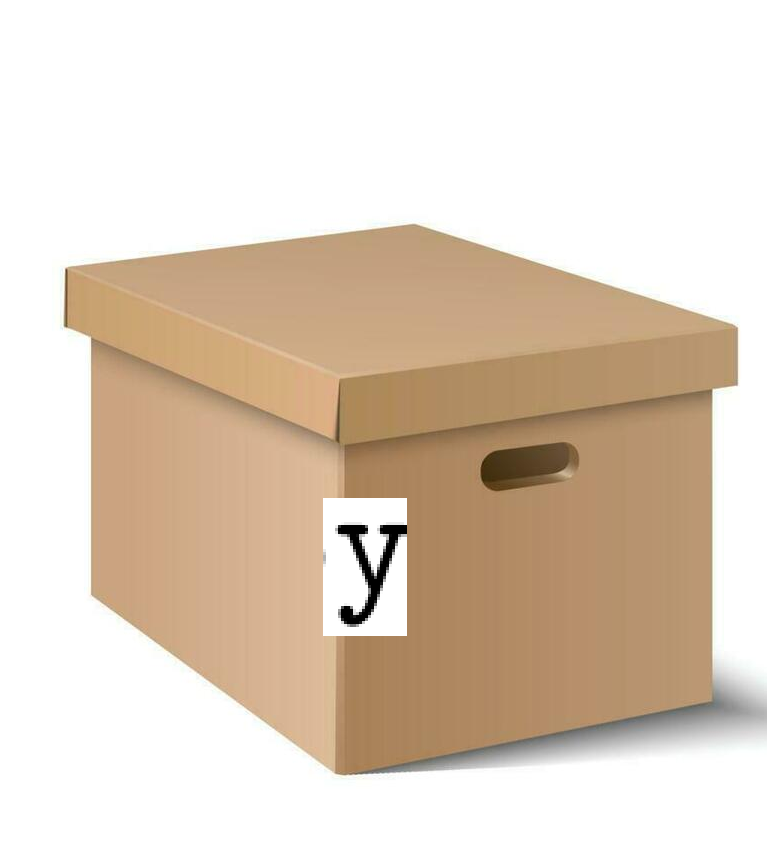
\includegraphics[width=3.6cm]{Images/Carton fermé_y.png}};
			}%
			% etape 9 : x s'ouvre, pointe vers 2 ; y reste ferme
			\only<9>{%
				\node (boitex) at (0,0) {
\includegraphics[width=3.6cm]{Images/Carton ouvert_x.png}};
				\node (boitey) at (5.5,0) {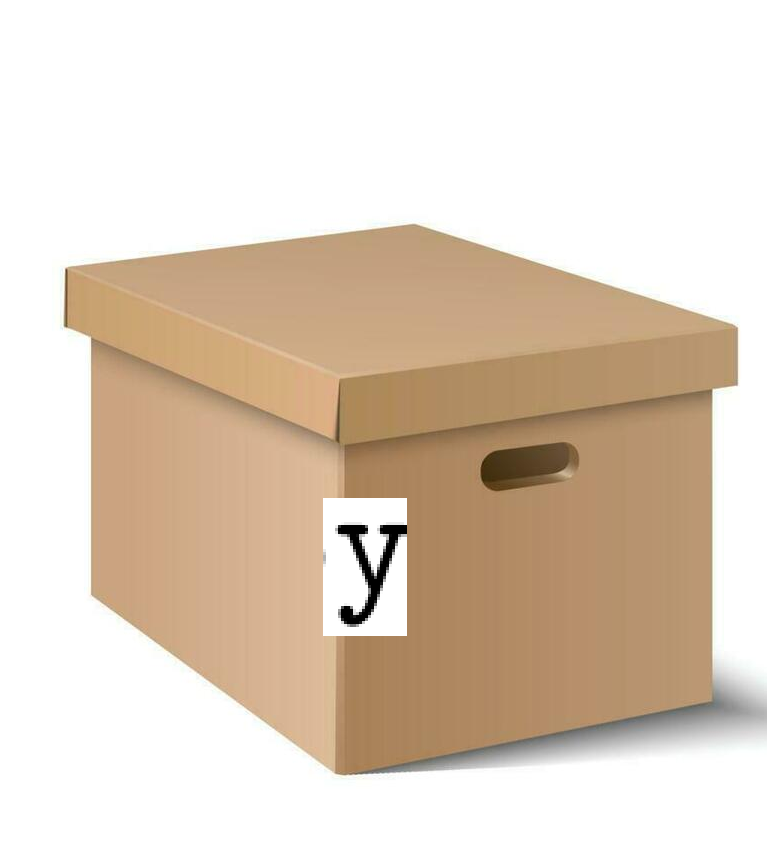
\includegraphics[width=3.6cm]{Images/Carton fermé_y.png}};
				\node[font=\Huge\bfseries] (deux) at ($(boitex.east)+(0.9,0.9)$) {2};
				\draw[-latex, thick] (boitex.east) to[bend left=15] (deux.west);
			}%
			% etape 10 : y s'ouvre aussi, pointe vers 3
			\only<10>{%
				\node (boitex) at (0,0) {
\includegraphics[width=3.6cm]{Images/Carton ouvert_x.png}};
				\node (boitey) at (5.5,0) {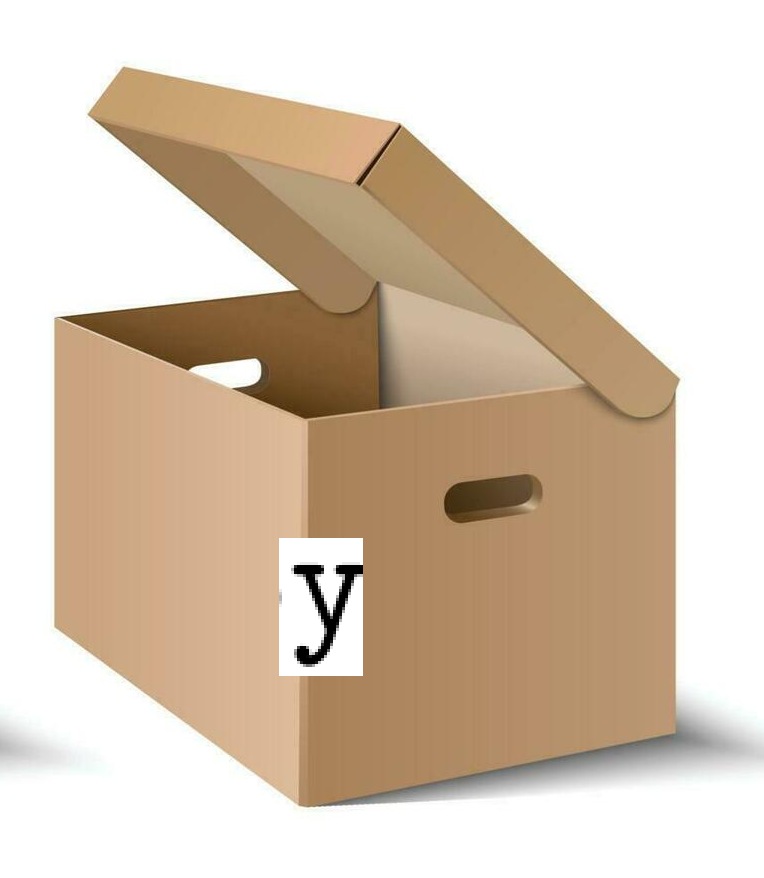
\includegraphics[width=3.6cm]{Images/Carton ouvert_y.png}};
				\node[font=\Huge\bfseries] (deux) at ($(boitex.east)+(0.9,0.9)$) {2};
				\draw[-latex, thick] (boitex.east) to[bend left=15] (deux.west);
				\node[font=\Huge\bfseries] (trois) at ($(boitey.east)+(0.9,0.9)$) {3};
				\draw[-latex, thick] (trois.west) to[bend right=15] (boitey.east);
			}%
			% etape 11 : nouveau depart, carton x ferme seul (y a disparu)
			\only<11>{\node (boite) at (0,0) {
\includegraphics[width=3.6cm]{Images/Carton fermé_x.png}};}%
			% etape 12 : x ouvert pointe vers 2, "Salut" apparait ailleurs, non relie
			\only<12>{%
				\node (boite) at (0,0) {
\includegraphics[width=3.6cm]{Images/Carton ouvert_x.png}};
				\node[font=\Huge\bfseries] (deux) at ($(boite.east)+(1.6,0.6)$) {2};
				\draw[-latex, thick] (boite.east) to[bend left=15] (deux.west);
				\node[font=\ttfamily\Large, text=codestr] (salut) at ($(boite.east)+(1.6,-1.3)$) {"Salut"};
			}%
			% etape 13 : la fleche vers 2 est barree, une nouvelle fleche vers "Salut" apparait
			\only<13>{%
				\node (boite) at (0,0) {
\includegraphics[width=3.6cm]{Images/Carton ouvert_x.png}};
				\node[font=\Huge\bfseries, black!45] (deux) at ($(boite.east)+(1.6,0.6)$) {2};
				\draw[-latex, thick, black!45] (boite.east) to[bend left=15] (deux.west);
				\draw[thick, red] ($(boite.east)!0.5!(deux.west)+(-0.25,-0.25)$) -- ($(boite.east)!0.5!(deux.west)+(0.25,0.25)$);
				\draw[thick, red] ($(boite.east)!0.5!(deux.west)+(-0.25,0.25)$) -- ($(boite.east)!0.5!(deux.west)+(0.25,-0.25)$);
				\node[font=\ttfamily\Large, text=codestr] (salut) at ($(boite.east)+(1.6,-1.3)$) {"Salut"};
				\draw[-latex, thick] (salut.west) to[bend left=15] (boite.east);
			}%
			% etape 14 : la fleche barree (et 2) disparaissent, "Salut" reste
			\only<14>{%
				\node (boite) at (0,0) {
\includegraphics[width=3.6cm]{Images/Carton ouvert_x.png}};
				\node[font=\ttfamily\Large, text=codestr] (salut) at ($(boite.east)+(1.6,-1.3)$) {"Salut"};
				\draw[-latex, thick] (salut.west) to[bend left=15] (boite.east);
			}%
			% etape 15 : le carton se referme
			\only<15>{%
				\node (boite) at (0,0) {
\includegraphics[width=3.6cm]{Images/Carton fermé_x.png}};
				\node[font=\ttfamily\Large, text=codestr] (salut) at ($(boite.east)+(1.6,-1.3)$) {"Salut"};
			}%
		\end{tikzpicture}
	\end{center}
\end{frame}

\begin{frame}[t]{Modèle mémoire de Python}
	
	\only<1>{\lstinputlisting[style=python,linerange={1-1}]{code/memoire_trace.py}}%
	\only<2-3>{\lstinputlisting[style=python,linerange={1-2}]{code/memoire_trace.py}}%
	\only<4->{\lstinputlisting[style=python,linerange={1-3}]{code/memoire_trace.py}}%
	
	\bigskip
	\begin{center}
		\begin{tikzpicture}[
			valbox/.style={draw, thick, rounded corners=2pt, minimum width=1.3cm, minimum height=0.9cm, font=\ttfamily},
			]
			% -- Pile : les noms --
			\draw[thick, rounded corners=2pt] (-0.4,-2.3) rectangle (3.1,0.5);
			\node[anchor=north west, font=\bfseries\footnotesize] at (-0.3,0.45) {Pile};
			
			\node[anchor=west, font=\ttfamily] (x) at (0.3,-0.5) {x};
			\onslide<2->{\node[anchor=west, font=\ttfamily] (y) at (0.3,-1.5) {y};}
			
			% -- Tas : les valeurs --
			\node[font=\itshape\footnotesize, black!60] at (7.1,0.75) {Tas};
			
			\node[valbox] (v42) at (7.1,-0.5) {42};
			\node[font=\itshape\tiny, black!55, above=1pt of v42] {int};
			
			\onslide<4->{
				\node[valbox] (v43) at (7.1,-2.1) {43};
				\node[font=\itshape\tiny, black!55, above=1pt of v43] {int};
			}
			
			% -- fleches (une reaffectation de x ne deplace pas la fleche de y !) --
			\only<1-3>{\draw[-latex, thick] (x.east) -- (v42.west);}
			% etape 2 : y pointe (a tort, pedagogiquement) directement vers x
			\only<2>{\draw[-latex, thick] (y.north) -- (x.south);}
			% etape 3+ : correction, y pointe vers l'objet vise par x, pas vers x lui-meme
			\onslide<3->{\draw[-latex, thick] (y.east) -- (v42.west);}
			\onslide<4->{\draw[-latex, thick] (x.east) -- (v43.west);}
		\end{tikzpicture}
	\end{center}
	
	\onslide<5->{
		\begin{center}
			\textbf{Réaffecter \texttt{x} ne change pas \texttt{y}.}
		\end{center}
	}
\end{frame}

% ===================================================================
% 5bis. Variables : definitions formelles
% ===================================================================

\begin{frame}{Variables : définitions}
	\begin{itemize}
		\item<2-> Une variable Python est un \textbf{nom} qui \textbf{référence} un objet.
		\medskip
		\item<3-> Le contenu de la variable est appelé la \textbf{valeur} de la variable.
		\medskip
		\item<4-> La syntaxe est :
		\begin{center}
			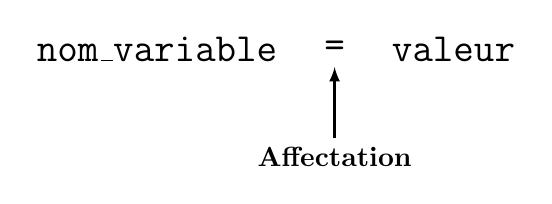
\begin{tikzpicture}[font=\ttfamily\Large]
				\node (nv) {nom\_variable};
				\node (eq) [right=0.35cm of nv] {=};
				\node (val) [right=0.35cm of eq] {valeur};
				\onslide<5->{
					\node[font=\normalsize\bfseries, below=0.9cm of eq] (aff) {Affectation};
					\draw[-latex, thick] (aff.north) -- (eq.south);
				}
			\end{tikzpicture}
		\end{center}
	\end{itemize}
\end{frame}

\begin{frame}{Choisir un nom de variable}
	\begin{itemize}
		\item<1-> Commence par une lettre (ou un tiret du bas \_)
		\medskip
		\item<2-> Pas d'espace ni de caractère spécial
		\medskip
		\item<3-> \emph{snake\_case} : \texttt{nom\_de\_variable}, et pas \texttt{nomdevariable} ou \texttt{NomDeVariable}
	\end{itemize}
	
	\onslide<4->{\bigskip\hrule\bigskip}
	
	\begin{itemize}
		\item<4-> Choisir un nom \textbf{clair}
	\end{itemize}
	
	\begin{center}
		\begin{tikzpicture}[font=\ttfamily\footnotesize]
			\onslide<4->{\node at (0,0) {\only<4>{t = 600}\only<5->{\sout{t = 600}}};}
			\onslide<5->{\node at (2.1,0) {\only<5>{taille = 600}\only<6->{\sout{taille = 600}}};}
			\onslide<6->{\node at (4.3,0) {\only<6>{lf = 600}\only<7->{\sout{lf = 600}}};}
			\onslide<7->{\node at (7.3,0) {largeur\_fenetre = 600};}
		\end{tikzpicture}
	\end{center}
	
	\begin{itemize}
		\item<8-> Souvent en anglais... mais français ok pour ce cours 
	\end{itemize}
\end{frame}

% ===================================================================
% 6. Transition : variables <-> valeurs
% ===================================================================

\begin{frame}[t]{Que peut-on mettre dans une variable ?}
	\only<1>{\lstinputlisting[
		style=pythonsmall,
		basicstyle=\ttfamily\scriptsize\color{black!45},
		keywordstyle=\color{black!45}, stringstyle=\color{black!45},
		emph={nb_notes,notes_entrees,listes_notes,nouvelle_note,liste_notes,nbre_notes,somme_notes,note,moyenne},
		emphstyle={\color{black}\bfseries},
		linebackgroundcolor={\color{white}%
			\ifnum\value{lstnumber}<4 \color{codekw!12}\fi
			\ifnum\value{lstnumber}=5 \color{codekw!12}\fi
			\ifnum\value{lstnumber}=10 \color{codekw!12}\fi
			\ifnum\value{lstnumber}=13 \color{codekw!12}\fi
			\ifnum\value{lstnumber}=15 \color{codekw!12}\fi
			\ifnum\value{lstnumber}=16 \color{codekw!12}\fi
			\ifnum\value{lstnumber}=19 \color{codekw!12}\fi
		},
		]{code/premier_prog_2.py}}%
	\only<2>{\lstinputlisting[
		style=pythonsmall,
		emph={nb_notes,notes_entrees,listes_notes,nouvelle_note,liste_notes,nbre_notes,somme_notes,note,moyenne},
		emphstyle={\color{black}\bfseries},
		linebackgroundcolor={\color{white}%
			\ifnum\value{lstnumber}<4 \color{codekw!12}\fi
			\ifnum\value{lstnumber}=5 \color{codekw!12}\fi
			\ifnum\value{lstnumber}=10 \color{codekw!12}\fi
			\ifnum\value{lstnumber}=13 \color{codekw!12}\fi
			\ifnum\value{lstnumber}=15 \color{codekw!12}\fi
			\ifnum\value{lstnumber}=16 \color{codekw!12}\fi
			\ifnum\value{lstnumber}=19 \color{codekw!12}\fi
		},
		]{code/focus_variables.py}}%
	
	% etapes 3-11 : le code disparait, des valeurs eparpillees apparaissent
	\only<3->{
		\begin{center}
			\begin{tikzpicture}[font=\small]
				\onslide<3->{\node at (-4.5,2.2) {Une note};}
				\onslide<4->{\node at (-1.2,2.4) {Une moyenne};}
				\onslide<5->{\node at (-4.5,1.0) {Un nombre de notes};}
				\onslide<6->{\node at (2.8,2.4) {\color{codestr}"Salut"};}
				\onslide<7->{\node at (-4.5,-0.2) {2};}
				\onslide<8->{\node at (0.8,-3.3) {Plein de notes différentes};}
				\onslide<9->{\node at (-1.2,-1.6) {Si on a fini de saisir};}
				\onslide<10->{\node at (2.8,1.0) {\color{codestr}"Entrez une note"};}
				\onslide<11->{\node at (2.8,-1.6) {Rien du tout};}
				
				% etape 12 : entiers
				\onslide<12->{
					\draw[thick, red, rounded corners=8pt] (-6.1,-0.7) rectangle (-3.0,2.7);
					\node[font=\bfseries] at (-4.55,-1.15) {Entiers : \texttt{int}};
				}
				% etape 13 : flottants (label sur 2 lignes pour ne pas deborder sur les chaines)
				\onslide<13->{
					\draw[thick, red, rounded corners=8pt] (-2.3,2.0) rectangle (-0.1,2.9);
					\node[font=\bfseries, anchor=north west, align=left] at (-2.9,1.85) {Nombres à virgule :\\\texttt{float}};
				}
				% etape 14 : booleens
				\onslide<14->{
					\draw[thick, red, rounded corners=8pt] (-2.7,-2.0) rectangle (0.3,-1.2);
					\node[font=\bfseries] at (-1.2,-2.4) {Vrai/Faux : \texttt{bool}};
				}
				% etape 15 : chaines de caracteres
				\onslide<15->{
					\draw[thick, red, rounded corners=8pt] (1.5,0.5) rectangle (4.4,2.9);
					\node[font=\bfseries] at (2.95,0.1) {Texte : \texttt{str}};
				}
				% etape 16-17 : NoneType (?? puis NoneType) - rectangle agrandi pour contenir tout le texte
				\onslide<16->{
					\draw[thick, red, rounded corners=8pt] (1.3,-2.0) rectangle (4.3,-1.2);
					\node[font=\bfseries] at (2.8,-2.4) {\only<16>{??}\only<17->{\texttt{NoneType}}};
				}
				% etape 18 : listes
				\onslide<18->{
					\draw[thick, red, rounded corners=8pt] (-2.2,-3.7) rectangle (3.8,-2.9);
					\node[font=\bfseries] at (0.8,-4.1) {Liste : \texttt{list}};
				}
			\end{tikzpicture}
		\end{center}
	}%
\end{frame}


% ===================================================================
% 7. Les types (sans faire une encyclopedie)
% ===================================================================

\begin{frame}{Quelques types de valeurs}
	\begin{center}
		\renewcommand{\arraystretch}{1.4}
		\begin{tabular}{lll}
			\texttt{int} & \texttt{42} & Nombre entier \\
			\texttt{float} & \texttt{3.14} & Nombre à virgule \\
			\texttt{str} & \texttt{"bonjour"}& Chaine de caractère \\
			\texttt{bool} & \texttt{True} & Booléen \\
			\texttt{NoneType} & \texttt{None} & Type vide \\
		\end{tabular}
	\end{center}
\end{frame}

% ===================================================================
% 7bis. Recap des types (exemples repris du notebook)
% ===================================================================

\begin{frame}[fragile]{Nombres entiers (\texttt{int})}
	\begin{lstlisting}[style=python]
		6
		12345
		-4                # un entier negatif
		2 ** 1000         # un tres tres grand entier
		0b101010          # ecriture binaire
		0x2a              # ecriture hexadecimale
	\end{lstlisting}
\end{frame}

\begin{frame}[fragile]{Nombres décimaux (\texttt{float})}
	\begin{lstlisting}[style=python]
		3.14
		-1.5
		12.
		4.56e3           # notation scientifique
	\end{lstlisting}
	\begin{center}
		\lstinputlisting[style=pythonoutput]{code/scientific_output.py}
	\end{center}
	\begin{lstlisting}
		3 * .1           # ne "tombe" pas toujours juste !
	\end{lstlisting}
	\begin{center}
		\lstinputlisting[style=pythonoutput]{code/tiers_output.py}
	\end{center}
\end{frame}

\begin{frame}[fragile]{Booléens (\texttt{bool})}
	\begin{lstlisting}[style=python]
		True
		False
		
		true             # attention a la casse !
	\end{lstlisting}
	\begin{center}
		\lstinputlisting[style=pythonoutput]{code/true_output.py}
	\end{center}
\end{frame}

\begin{frame}[fragile]{Chaînes de caractères (\texttt{str})}
	\begin{lstlisting}[style=python]
		'bonjour'                    # guillemets simples
		"hello !"                    # guillemets doubles
		"""Un texte
		sur plusieurs lignes"""      # chaine longue
		"King's Landing"             # une apostrophe a l'interieur
		"sauts\nde\nligne"           # caracteres speciaux
	\end{lstlisting}
\end{frame}

\begin{frame}[fragile]{Valeur indéfinie (\texttt{NoneType})}
	\begin{lstlisting}[style=python]
		None
	\end{lstlisting}
\end{frame}

% ===================================================================
% 7ter. Operateurs
% ===================================================================

\begin{frame}[fragile]{Opérations sur les nombres}
	\begin{lstlisting}[style=python]
		4 + 5
		4 - 5.5
		4. * 5.
		4 ** 2
		4 ** 0.5
	\end{lstlisting}
	\bigskip
	\begin{lstlisting}[style=python]
		4 + 2 * 1.5          # priorites usuelles
		(4 + 2) * 1.5        # ... et les parentheses
	\end{lstlisting}
\end{frame}

\begin{frame}[fragile]{Division}
	\begin{lstlisting}[style=python]
		1 / 3          # division reelle : toujours un float
		4 / 2          # ... meme ici : 2.0 !
		7 // 2         # quotient (division euclidienne)
		7 % 2          # reste
		divmod(7, 2)   # les deux a la fois
	\end{lstlisting}
\end{frame}

\begin{frame}[fragile]{Opérations sur les chaînes de caractères}
	\begin{lstlisting}[style=python]
		'Gustave' + 'Eiffel'
		'Gustave' + ' ' + 'Eiffel'
		'Hip ' * 3 + 'Hourra !'
	\end{lstlisting}
	\bigskip
	\begin{center}
		\emph{Attention : \texttt{+} et \texttt{*} n'ont pas le même sens sur des chaînes et sur des nombres !}
	\end{center}
\end{frame}

% ===================================================================
% 7quater. Tableau de valeurs
% ===================================================================

\begin{frame}[t]{Un tableau de valeurs}
	\begin{columns}[T]
		\begin{column}{0.55\textwidth}
			\only<1>{\valline{code/echange_valeurs.py}{1-1}{1}\valline{code/echange_valeurs.py}{2-5}{0}}%
			\only<2>{\valline{code/echange_valeurs.py}{1-1}{0}\valline{code/echange_valeurs.py}{2-2}{1}\valline{code/echange_valeurs.py}{3-5}{0}}%
			\only<3>{\valline{code/echange_valeurs.py}{1-2}{0}\valline{code/echange_valeurs.py}{3-3}{1}\valline{code/echange_valeurs.py}{4-5}{0}}%
			\only<4>{\valline{code/echange_valeurs.py}{1-3}{0}\valline{code/echange_valeurs.py}{4-4}{1}\valline{code/echange_valeurs.py}{5-5}{0}}%
			\only<5->{\valline{code/echange_valeurs.py}{1-4}{0}\valline{code/echange_valeurs.py}{5-5}{1}}%
		\end{column}
		\begin{column}{0.4\textwidth}
			\begin{center}
				\renewcommand{\arraystretch}{1.3}
				\begin{tabular}{cc}
					\texttt{a} & \texttt{b} \\ \hline
					\onslide<1->{\texttt{3} & \texttt{---} \\}
					\onslide<2->{\texttt{3} & \texttt{5} \\}
					\onslide<3->{\texttt{8} & \texttt{5} \\}
					\onslide<4->{\texttt{8} & \texttt{3} \\}
					\onslide<5->{\texttt{5} & \texttt{3} \\}
				\end{tabular}
			\end{center}
		\end{column}
	\end{columns}
	\onslide<6->{
		\begin{center}
			\textbf{On a échangé les deux valeurs, sans variable auxiliaire !}
		\end{center}
	}
\end{frame}

\iffalse % --- reste du brouillon desactive le temps de travailler la slide 1 ---
% ===================================================================
% 8. Activite turtle : dessin de polygone
% ===================================================================

\begin{frame}[fragile]{Activité : dessiner un polygone}
	\begin{lstlisting}[style=python]
		import turtle
		
		t = turtle.Turtle()
		for i in range(5):
		t.forward(100)
		t.left(72)
	\end{lstlisting}
\end{frame}

% ===================================================================
% 9. Tableau de valeurs (PLACEHOLDER - a adapter au contenu reel du TD)
% ===================================================================

\begin{frame}{Notes de la classe}
	\begin{center}
		\renewcommand{\arraystretch}{1.3}
		\begin{tabular}{lc}
			Étudiant·e & Moyenne \\ \hline
			Alice & 14.5 \\
			Bilal & 9.0 \\
			Chloé & 17.25 \\
			David & 11.0 \\
		\end{tabular}
	\end{center}
\end{frame}

\fi % --- fin du bloc desactive ---

\end{document}
